%!TEX root = ../2019_06_04-HATS-LPC-JEC.tex

\subsection{Pileup Mitigation}
%---------------------------------------------------------------------------------------------------------------------------------------
\begin{frame}
    \begin{block}{}
        \begin{center}
            \shadowoffset{2pt}
            \shadowcolor{CUGold}
            \shadowtext{{\fontsize{30}{60}\selectfont \textbf{\textcolor{black}{Pileup Mitigation}}}}
            \vspace{1.5mm}
        \end{center}
    \end{block}
\end{frame}

\begin{frame}[t]\frametitle{CMS Event Reconstruction -- Abbreviated}    
	\begin{textblock}{0.4}(0.03,0.12)
		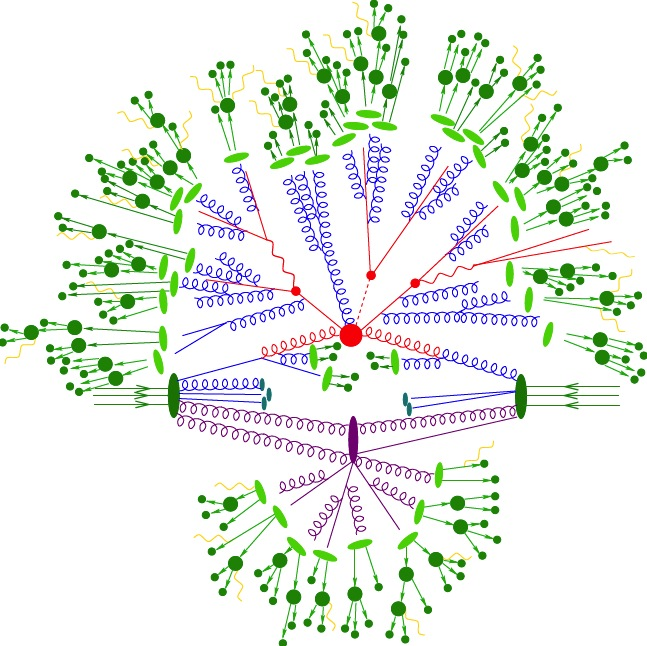
\includegraphics[width=\textwidth]{images/pileup_mitigation/sherpa_sim_0.jpeg}
	\end{textblock}
	\begin{textblock}{0.3}(0.02,0.48)
		\tiny
		{\color{red}Hard Process}\\
		{\color{blue}Parton Showers}\\
		{\color{violet}Underlying Event}\\
		{\color{green}Hadronization}\\
		{\color{ForestGreen}Hadron Decay}\\
		{\color{CUGold}QED}
	\end{textblock}   
	\begin{textblock}{0.55}(0.45,0.1)
		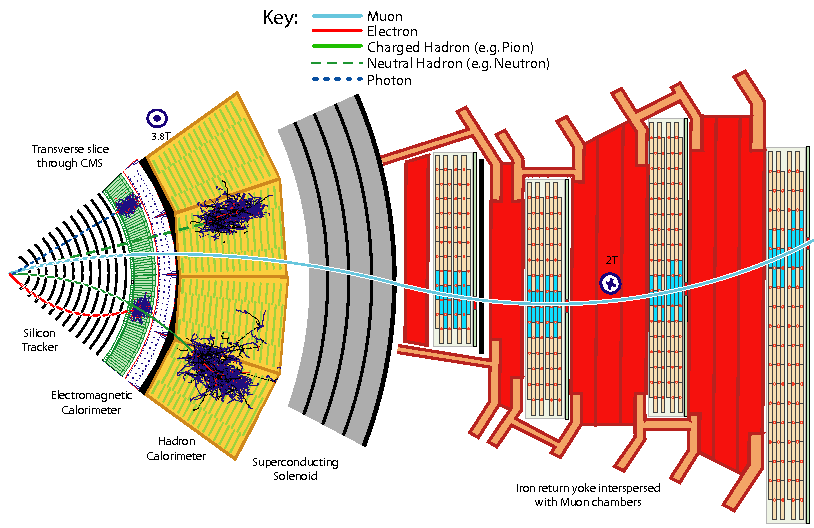
\includegraphics[width=\textwidth]{images/pileup_mitigation/cms-transverse-slice-crop.png}
	\end{textblock}
	\begin{textblock}{0.5}(0.5,0.565)
		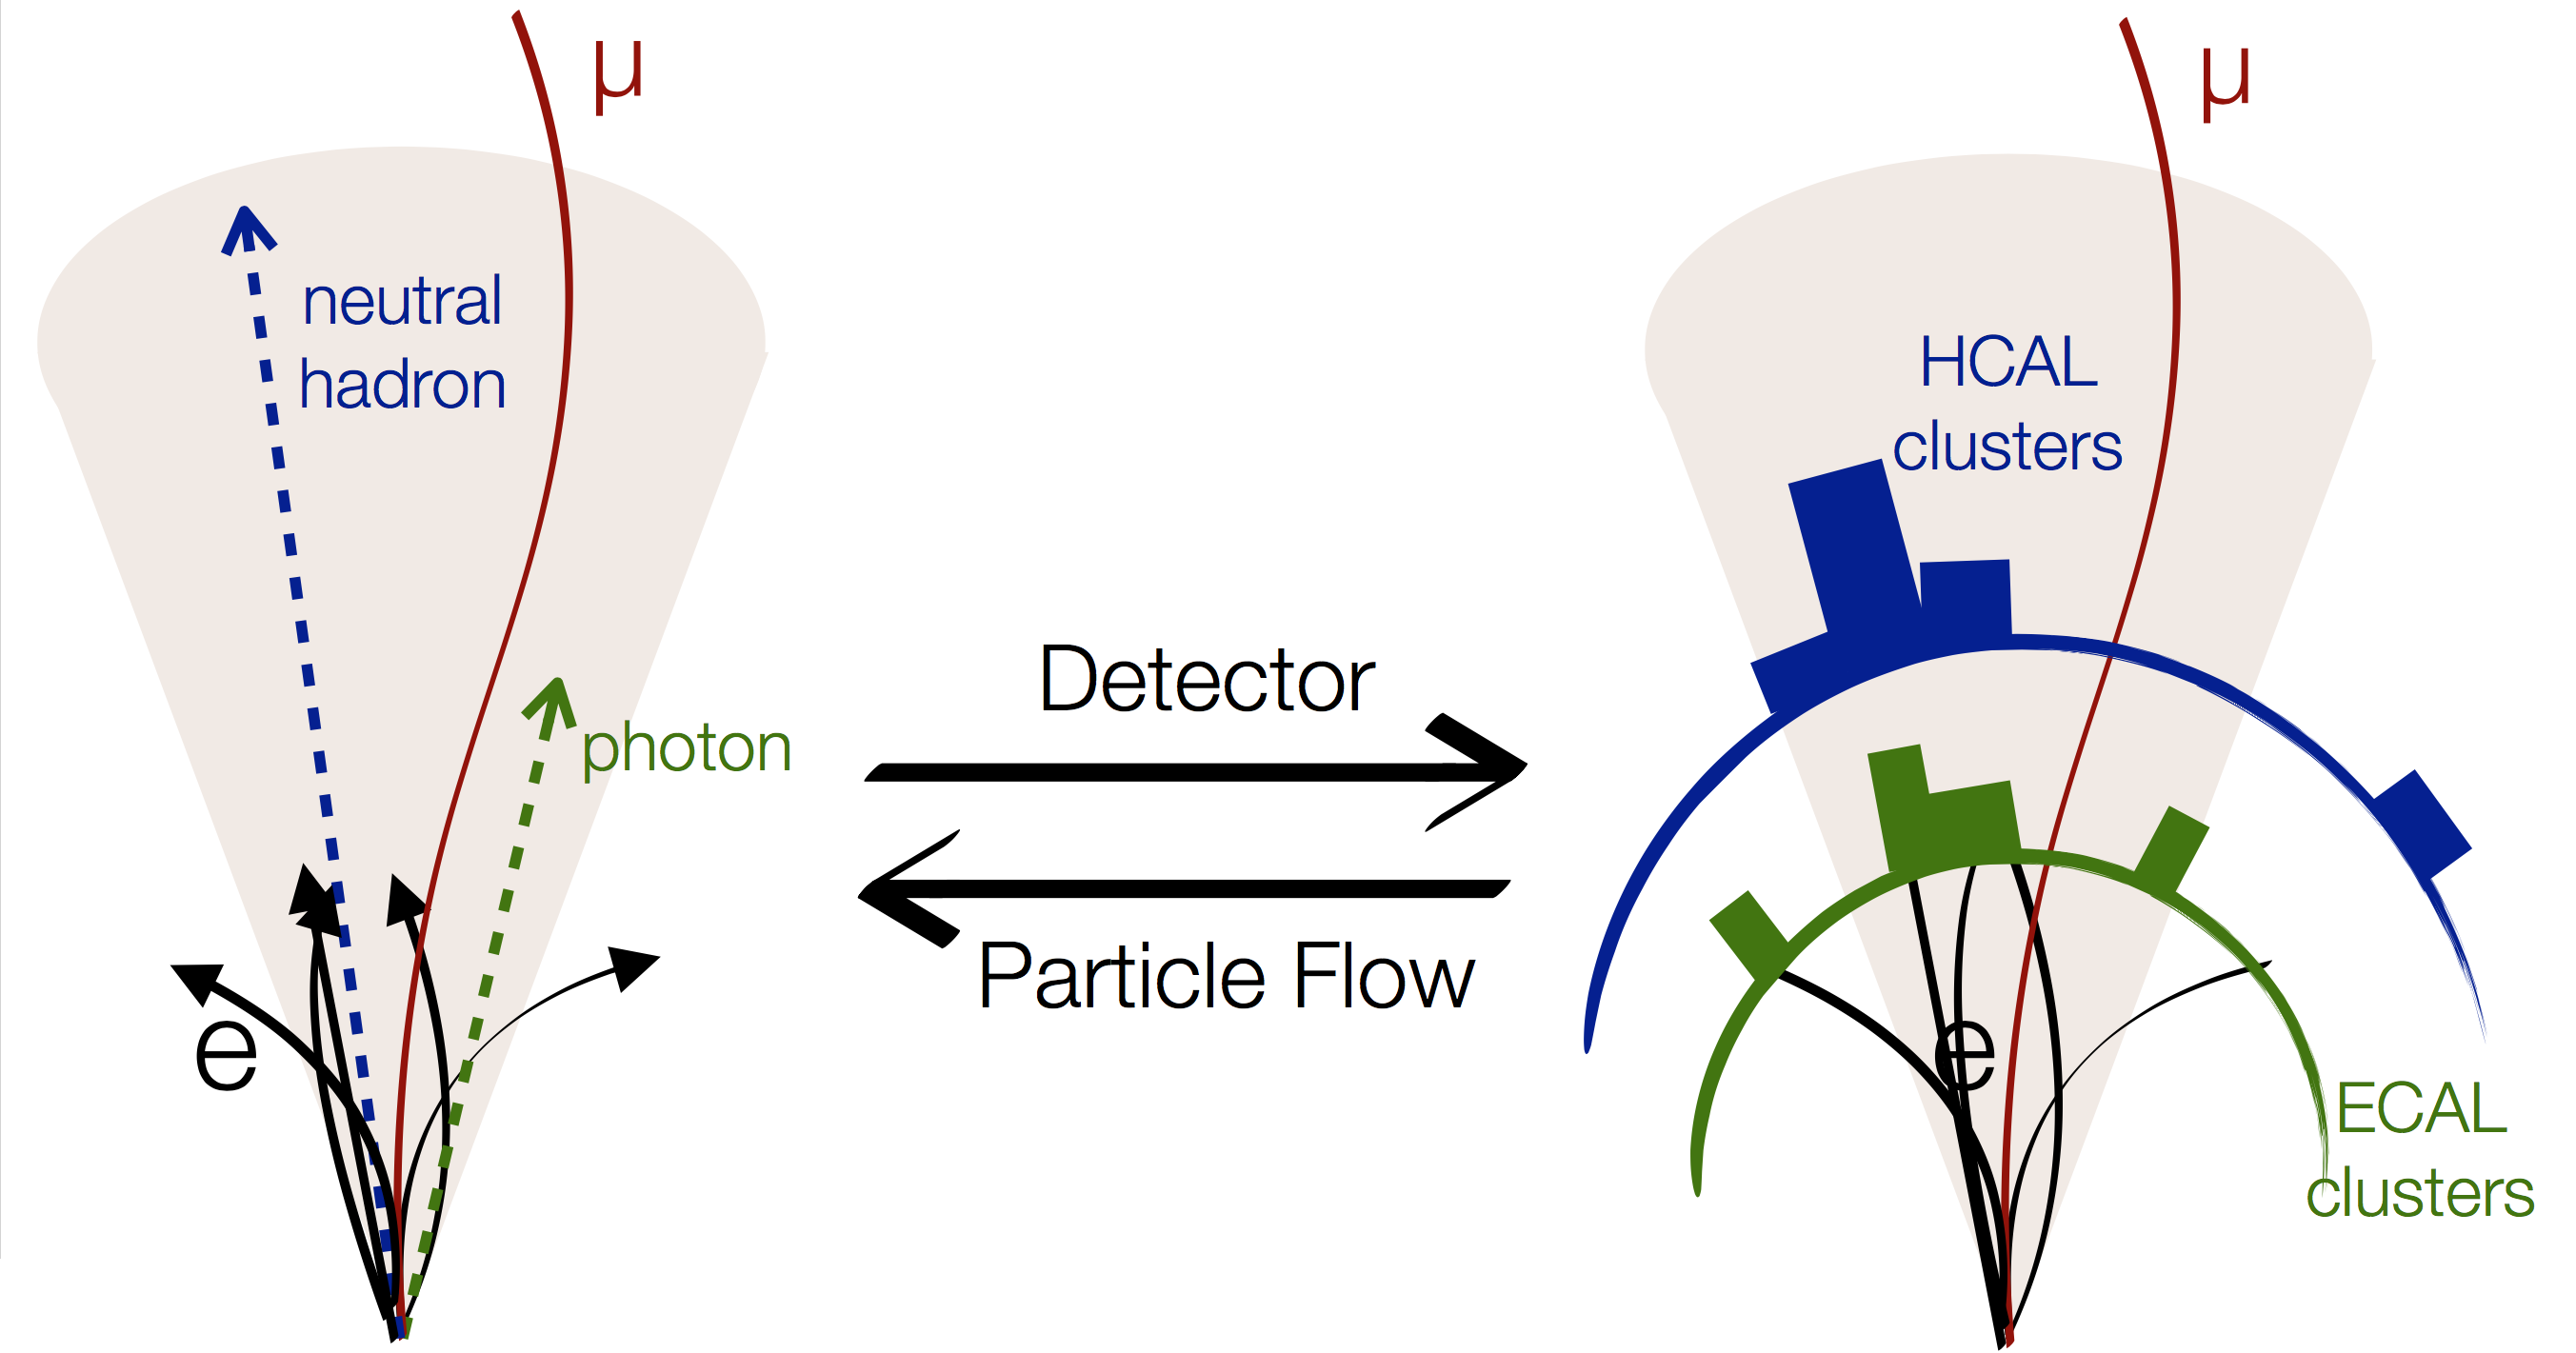
\includegraphics[width=\textwidth]{images/pileup_mitigation/PFAlgo.png}
	\end{textblock}
	\begin{textblock}{0.4}(0.06,0.68)
		\centering
		\ul{Particle Flow Reconstruction}
		\vspace*{0.2cm}

		{\color{maroon}
		calorimeter clusters and tracks$\Rightarrow$
		\vspace*{0.2cm}

		muons, electrons, photons, neutral hadrons, charged hadrons}
	\end{textblock}
\end{frame}

\begin{frame}[t]\frametitle{What does an event look like?}
	\vspace*{0.25cm}
	\begin{figure}[tb]
		\centering
		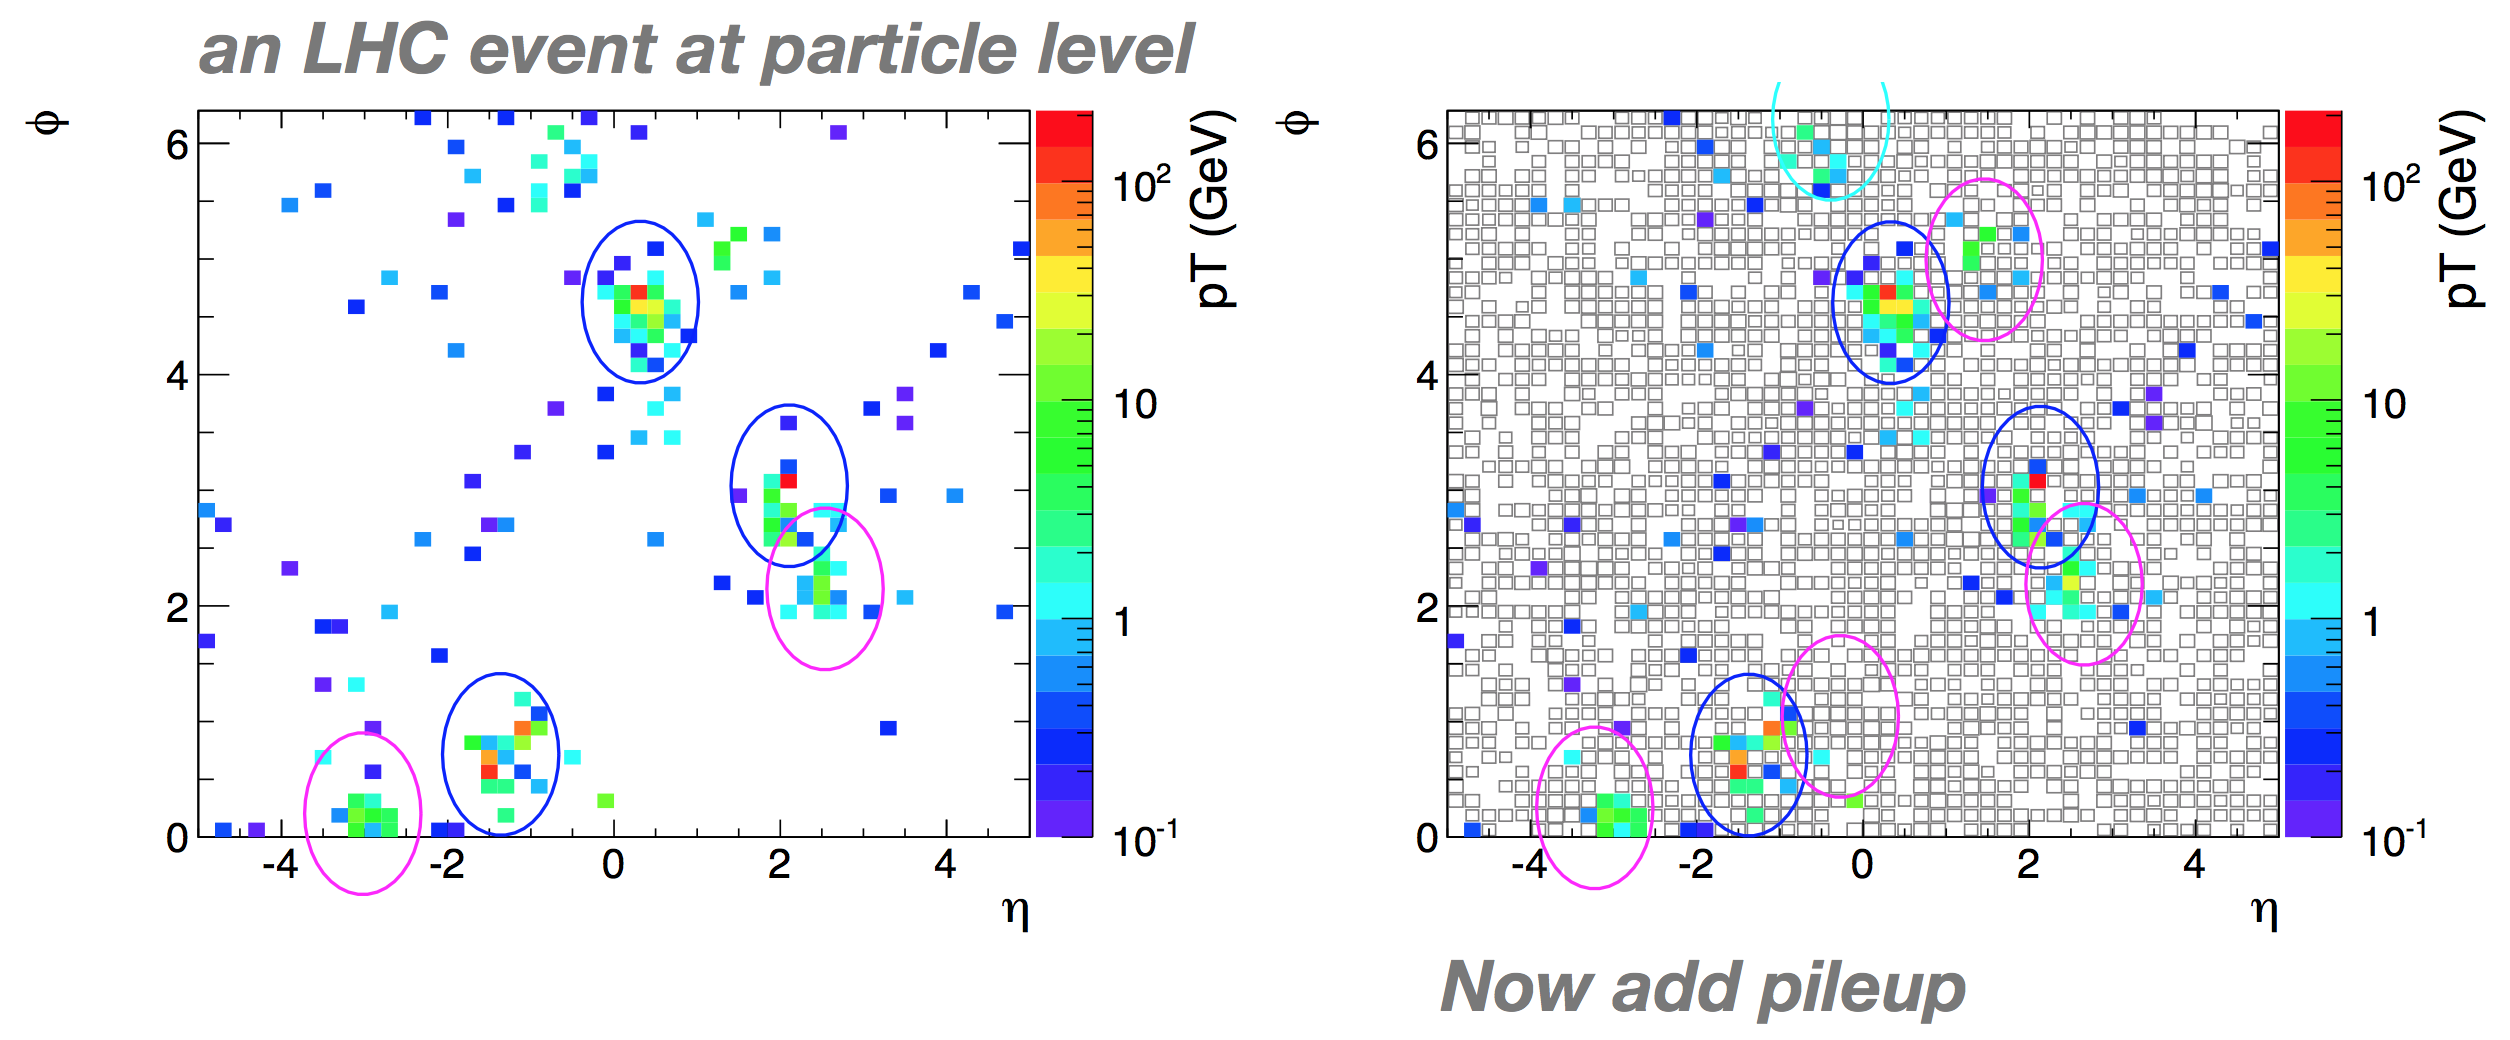
\includegraphics[width=\textwidth]{images/pileup_mitigation/LHC_event_particle_level.png}
	\end{figure}
\end{frame}

\begin{frame}[t]\frametitle{Pileup Mitigation}
	\vspace*{-0.35cm}
	\begin{block}{}
		\vbox to .88\vsize{
		\begin{customlist}{2.5em}{0em}
		   \item Many clever ways have been devised to remove the effects of pileup from physics analyses and objects
		   \item Some (basic) techniques that have been used for several years:
		   \begin{enumerate}
		      \item {\color{RoyalBlue}PFchs a.k.a. PFnoPU a.k.a. ...}
		      \begin{itemize}
		      	\item Specific subtraction of charged energy from pileup
		      \end{itemize}
		      \item {\color{RoyalBlue}L1FastJet}
		      \begin{itemize}
		      	\item Global subtraction of average energy density, $\rho$
		      \end{itemize}
		      \item {\color{RoyalBlue}$\beta$, $\Delta\beta$}
		      \begin{itemize}
		      	\item Alternate methods for isolation treatment (not discussed today)
		      \end{itemize}
		   \end{enumerate}
		   \item Pileup affects all objects (MET, muons, etc.). we are focusing on jets today
		\end{customlist}
		}
	\end{block}
\end{frame}

\begin{frame}[t]\frametitle{Charged Hadron Subtraction}
    \vspace*{-0.45cm}
    \begin{columns}[T]
    	\begin{column}{0.58\textwidth}
	    	Tracking is a major tool -- we can identify most charged particles from non-leading primary vertices

	    	\begin{center}
	    		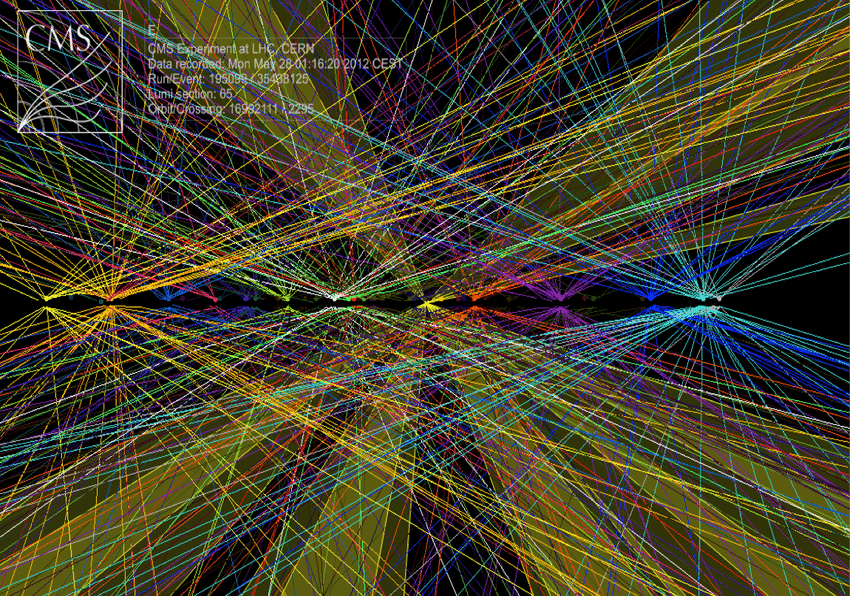
\includegraphics[width=0.8\textwidth]{images/pileup_mitigation/pileup-vertices-colored.png}
	    	\end{center}

    		Leading primary vertex has largest $\sum |p_{T}^{track}|^{2}$\\
    		\vspace*{0.2cm}
    		$\Rightarrow$ Remove tracks from non-leading (aka pileup) vertices before clustering jets
    	\end{column}
    	\begin{column}{0.38\textwidth}
    		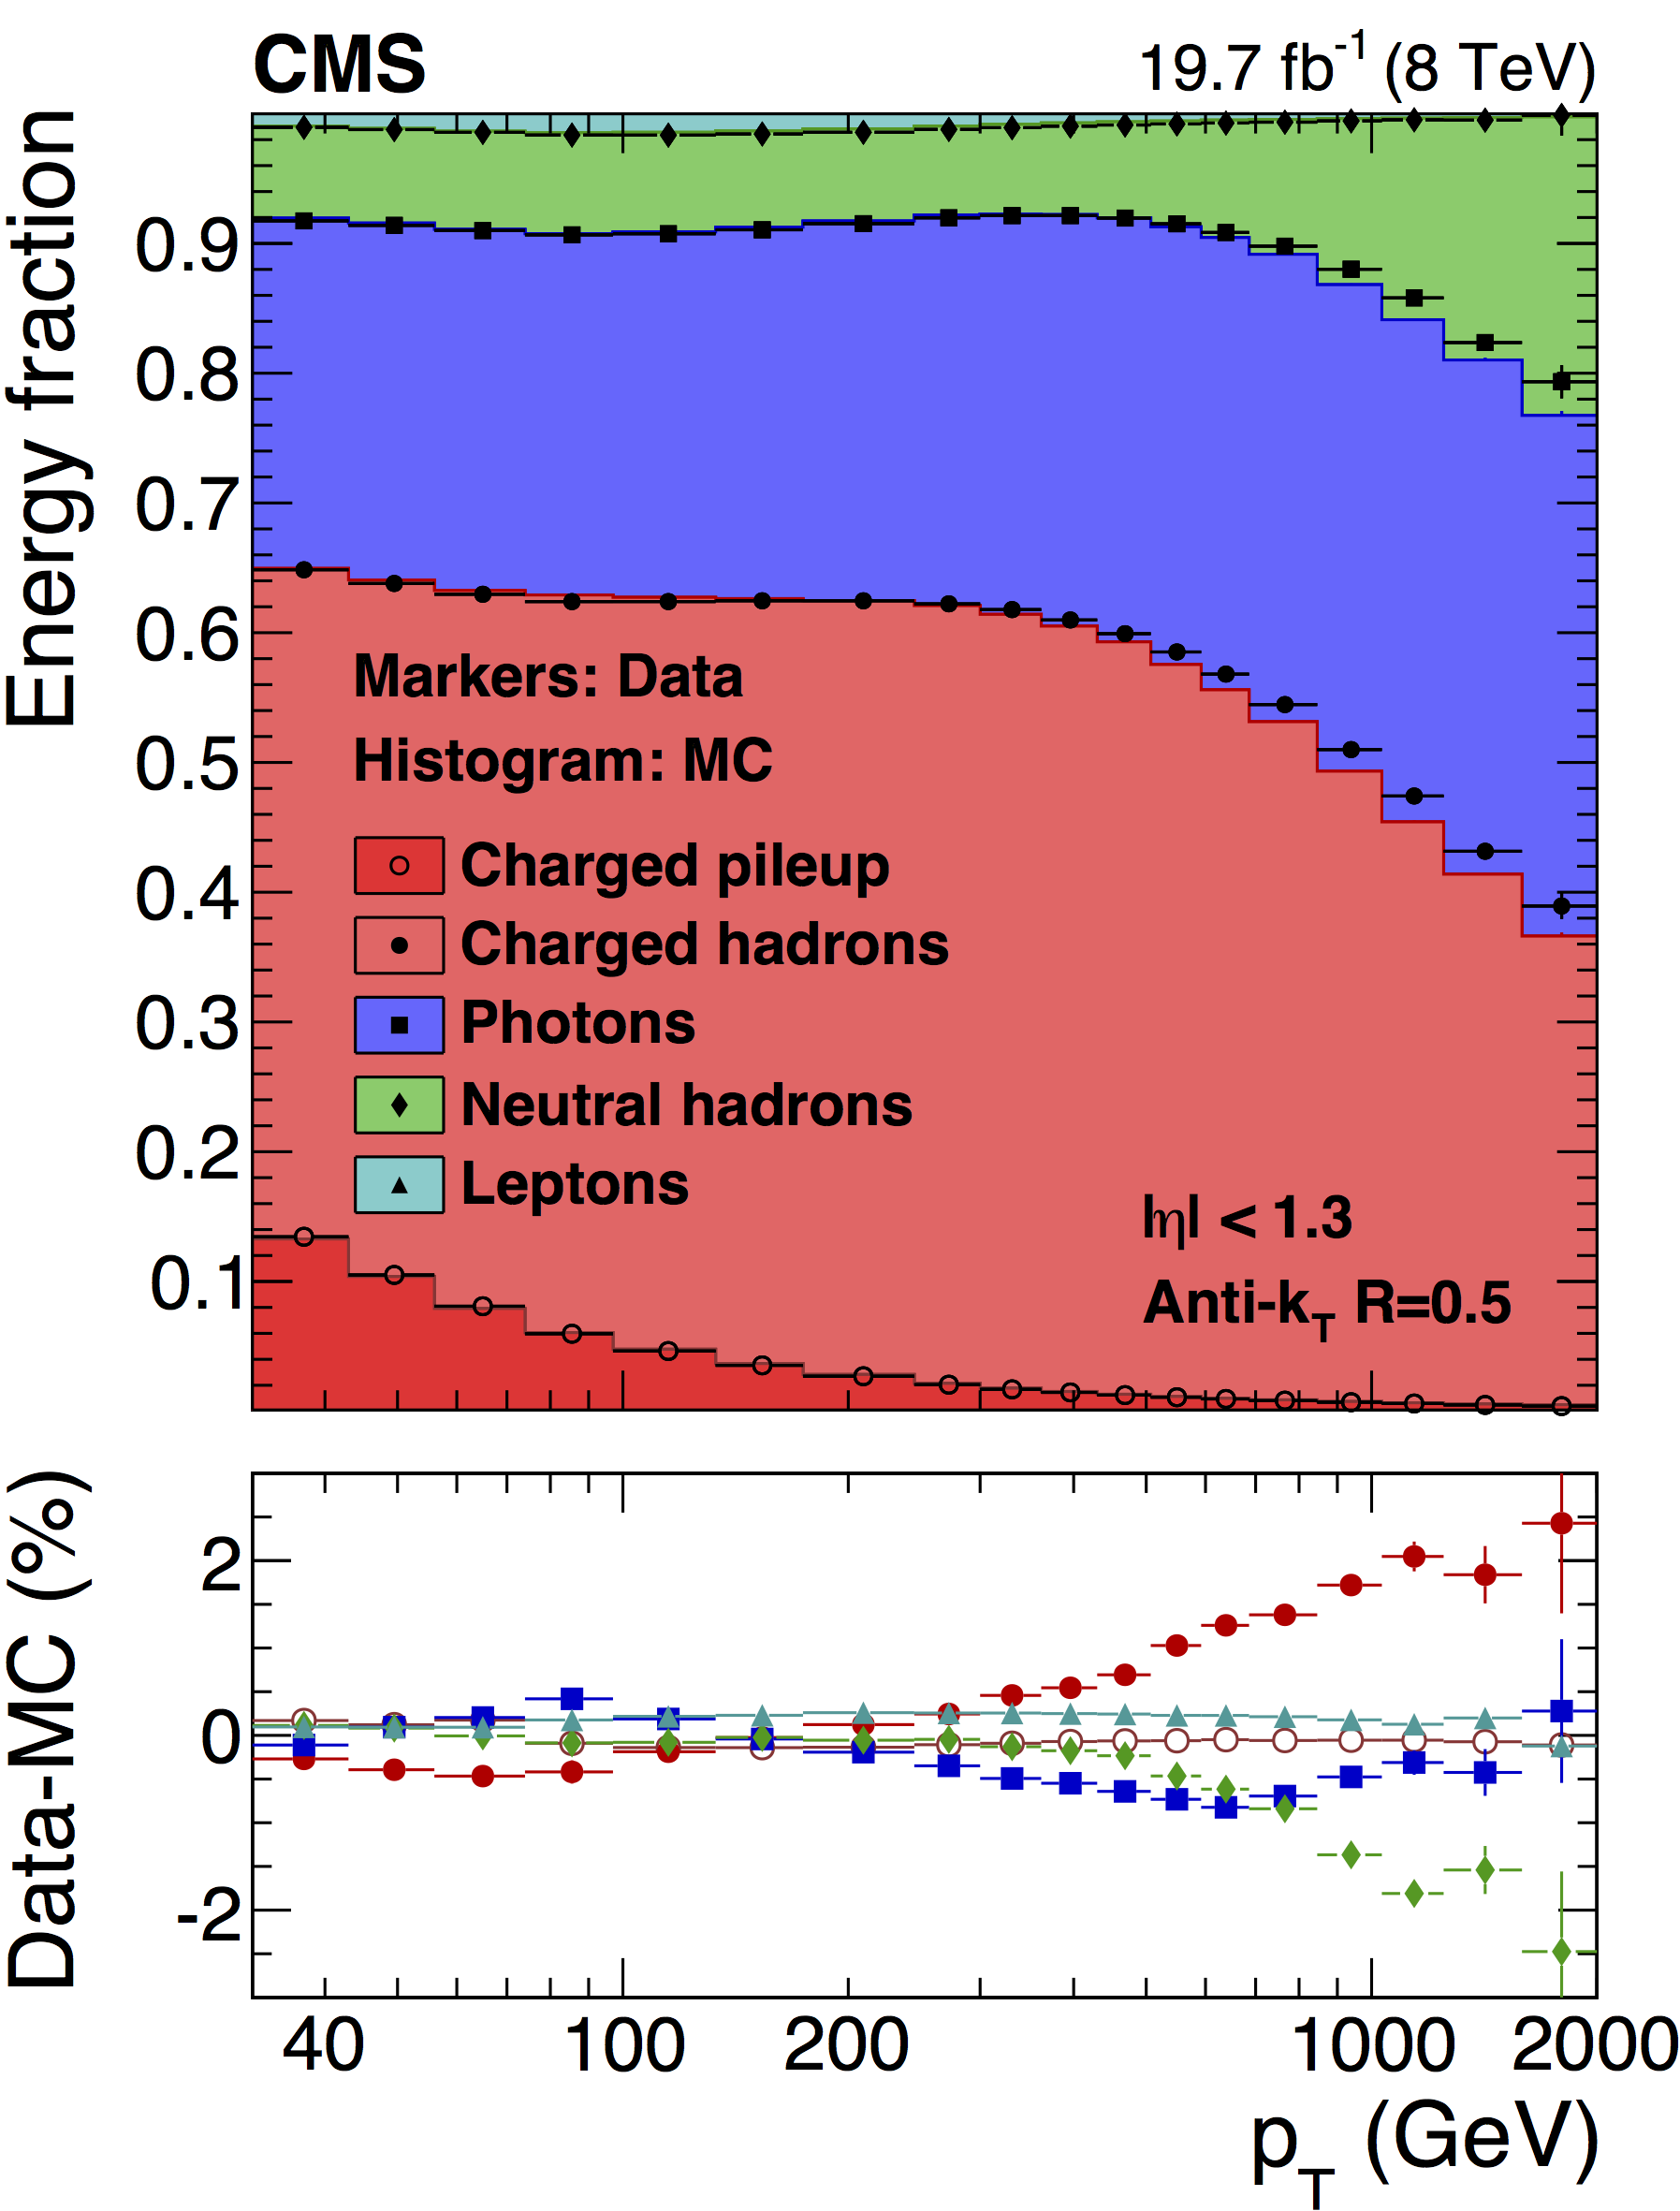
\includegraphics[width=\textwidth]{images/pileup_mitigation/composition_combo_pt_pfpaper_final_v2.png}
    	\end{column}
    \end{columns}
\end{frame}

\begin{frame}[t]\frametitle{$\rho$ Pileup Correction}
	\vspace*{-0.35cm}
	Imagine making a grid out of your detector\\
	~~$\Rightarrow\rho$ is the median patch value ($p_{T}/area$)
	\begin{figure}[tb]
		\hspace*{-3cm}
		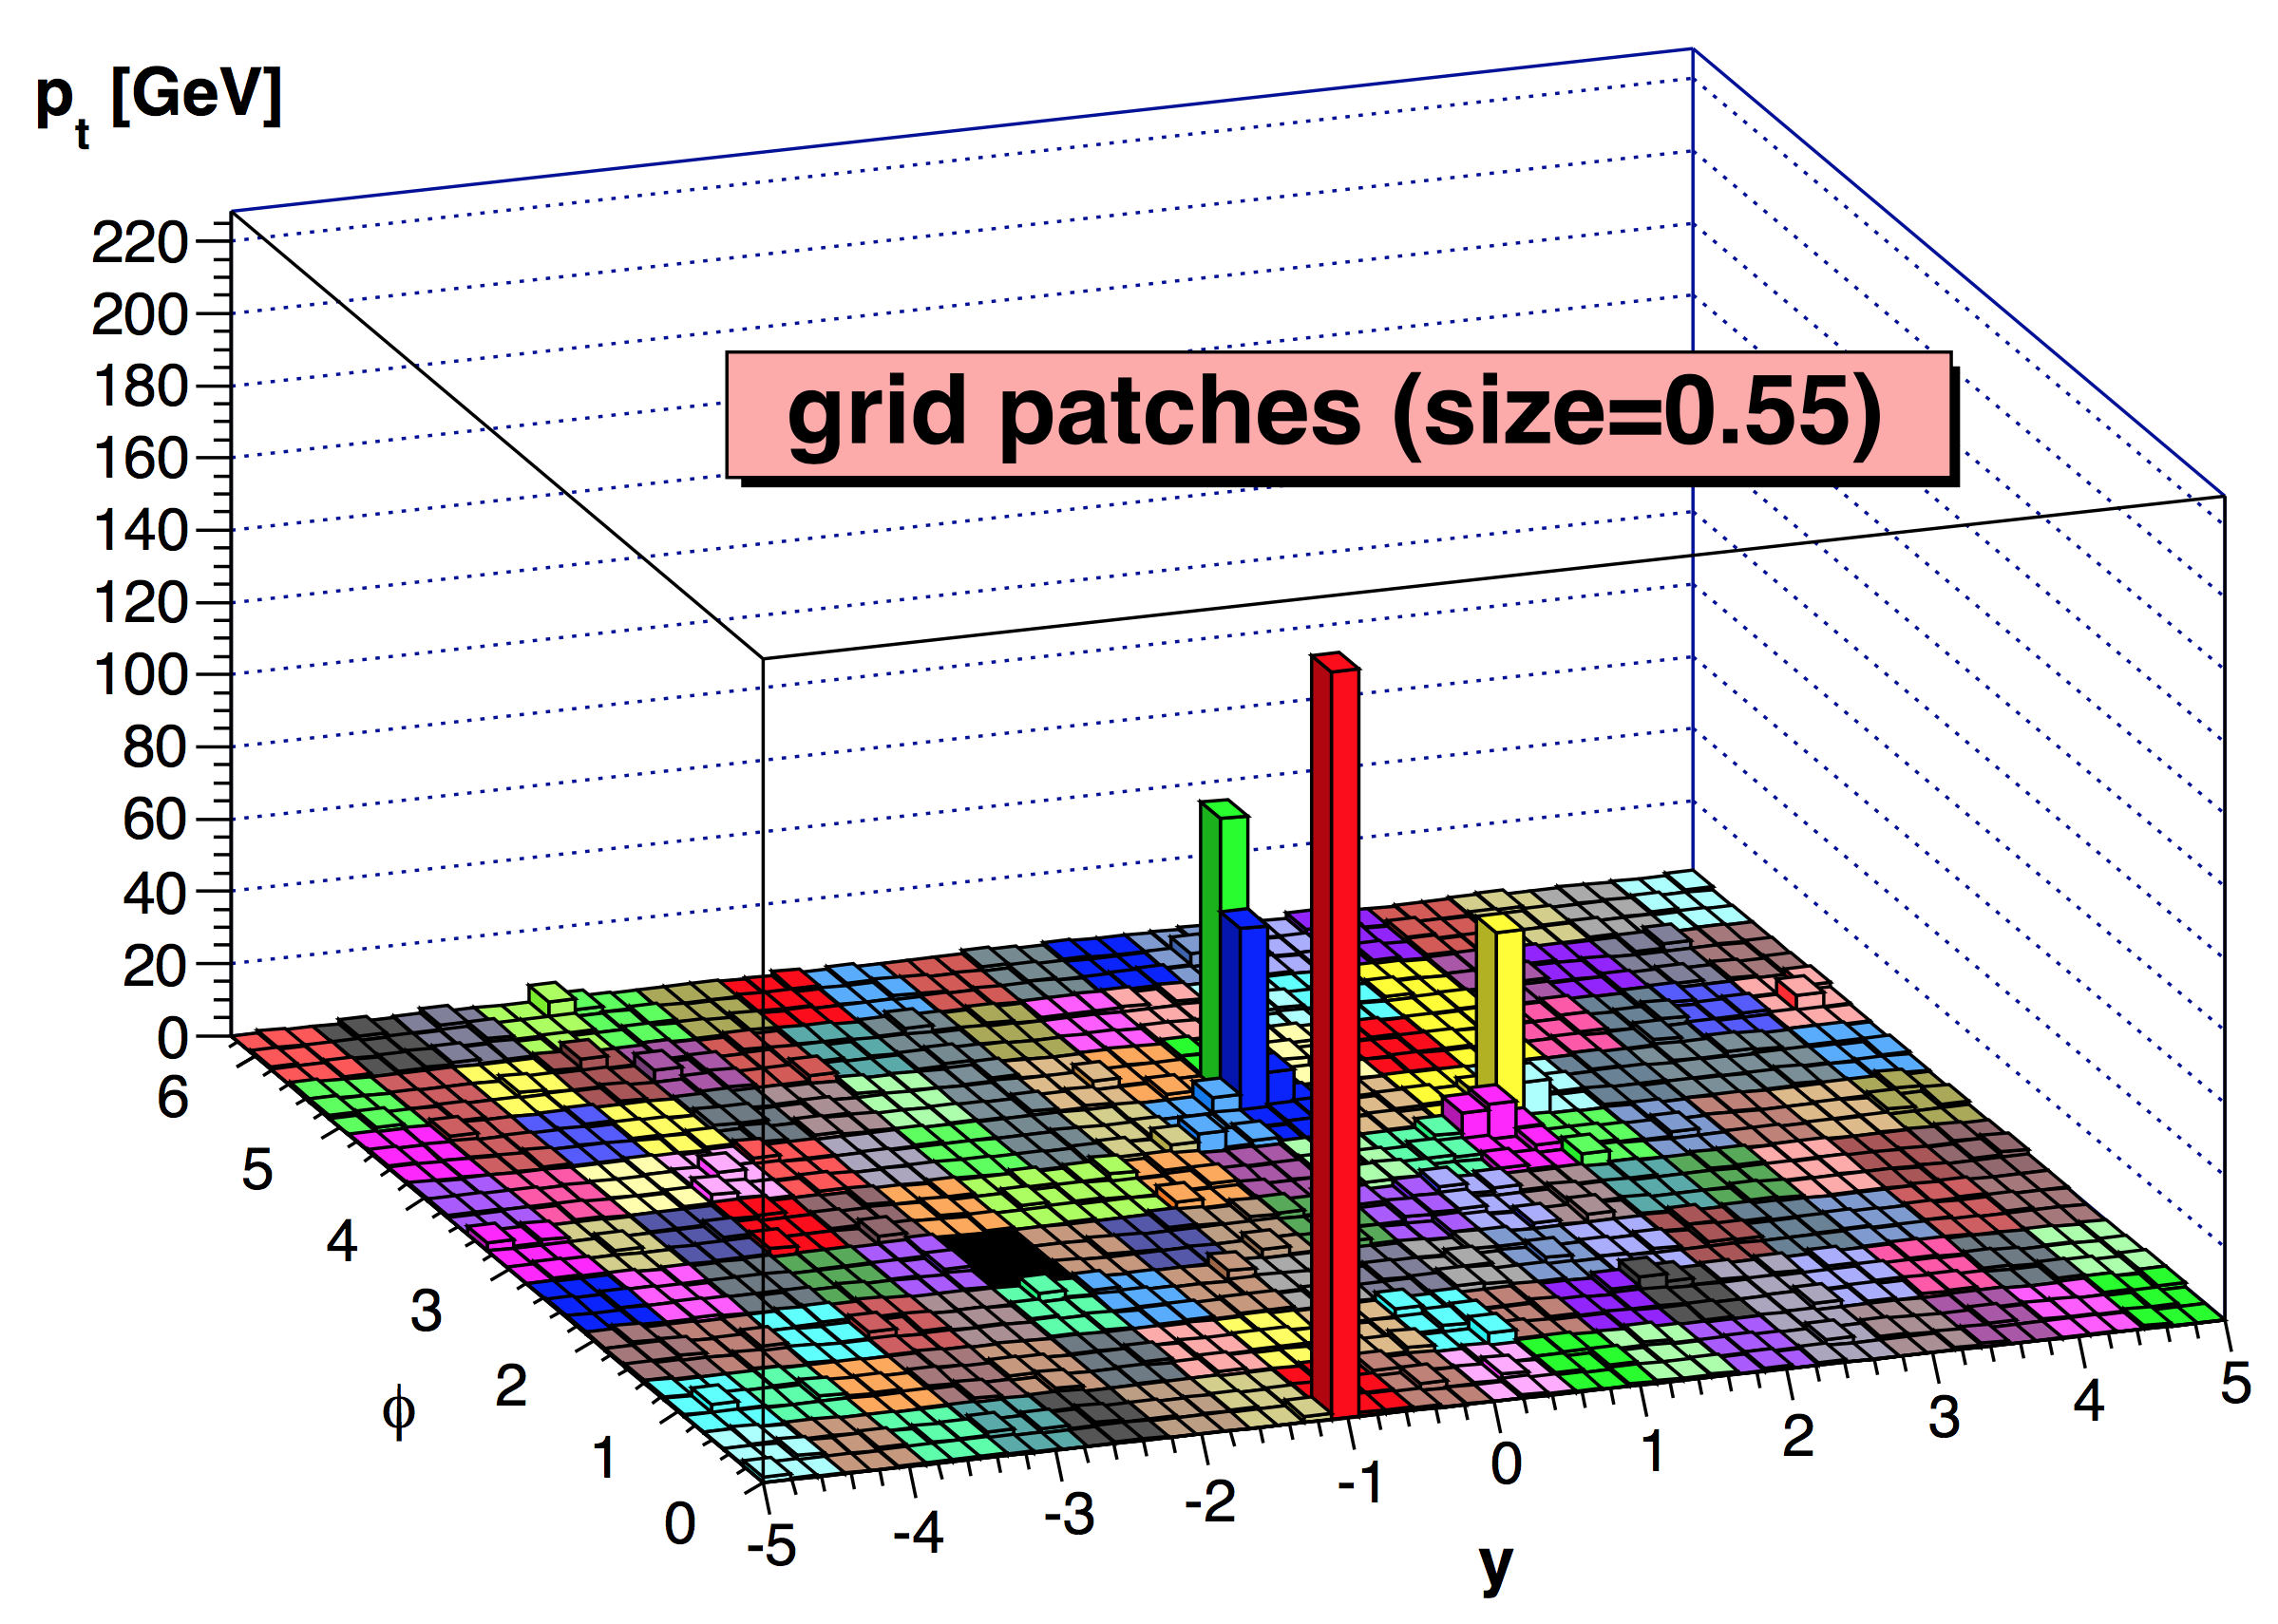
\includegraphics[width=0.6\textwidth]{images/pileup_mitigation/rho.png}
	\end{figure}
	\begin{textblock}{0.4}(0.62,0.3)
		N.B. there is an $\eta$ dependence
	\end{textblock}
	\textbf{How to correct jets:} $p_{T}^{corr}=p_{T}^{raw}-\rho\times A$\\
	\vspace*{0.15cm}
	N.B. this is done for data and for MC
\end{frame}

\begin{frame}<1>[t,label=frame:pileup_schematic]\frametitle{\only<1>{$\rho$ Pileup Correction}\only<2-3>{Pileup Correction}}
	\begin{textblock}{0.96}(0.02,0.3)
			\only<1-2>{
				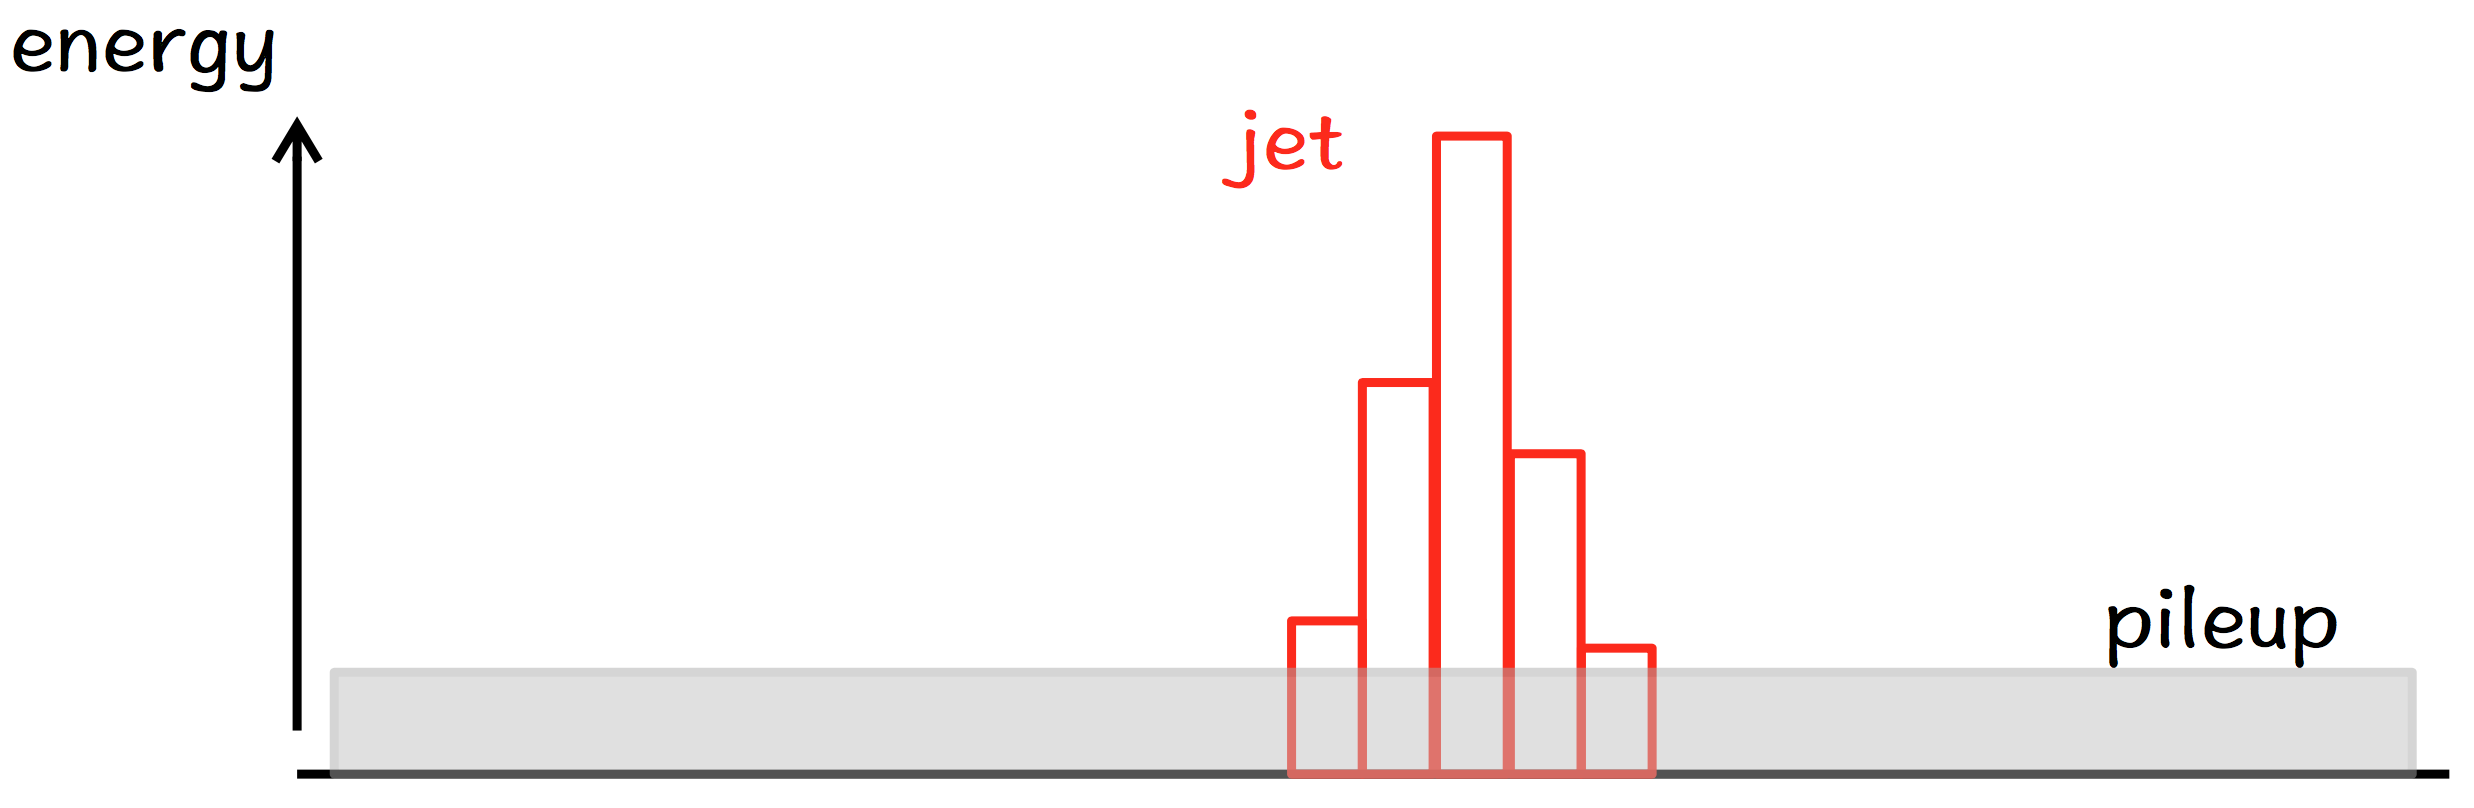
\includegraphics[width=\textwidth]{images/pileup_mitigation/pileup_schematic_1.png}
			}
			\only<3>{
				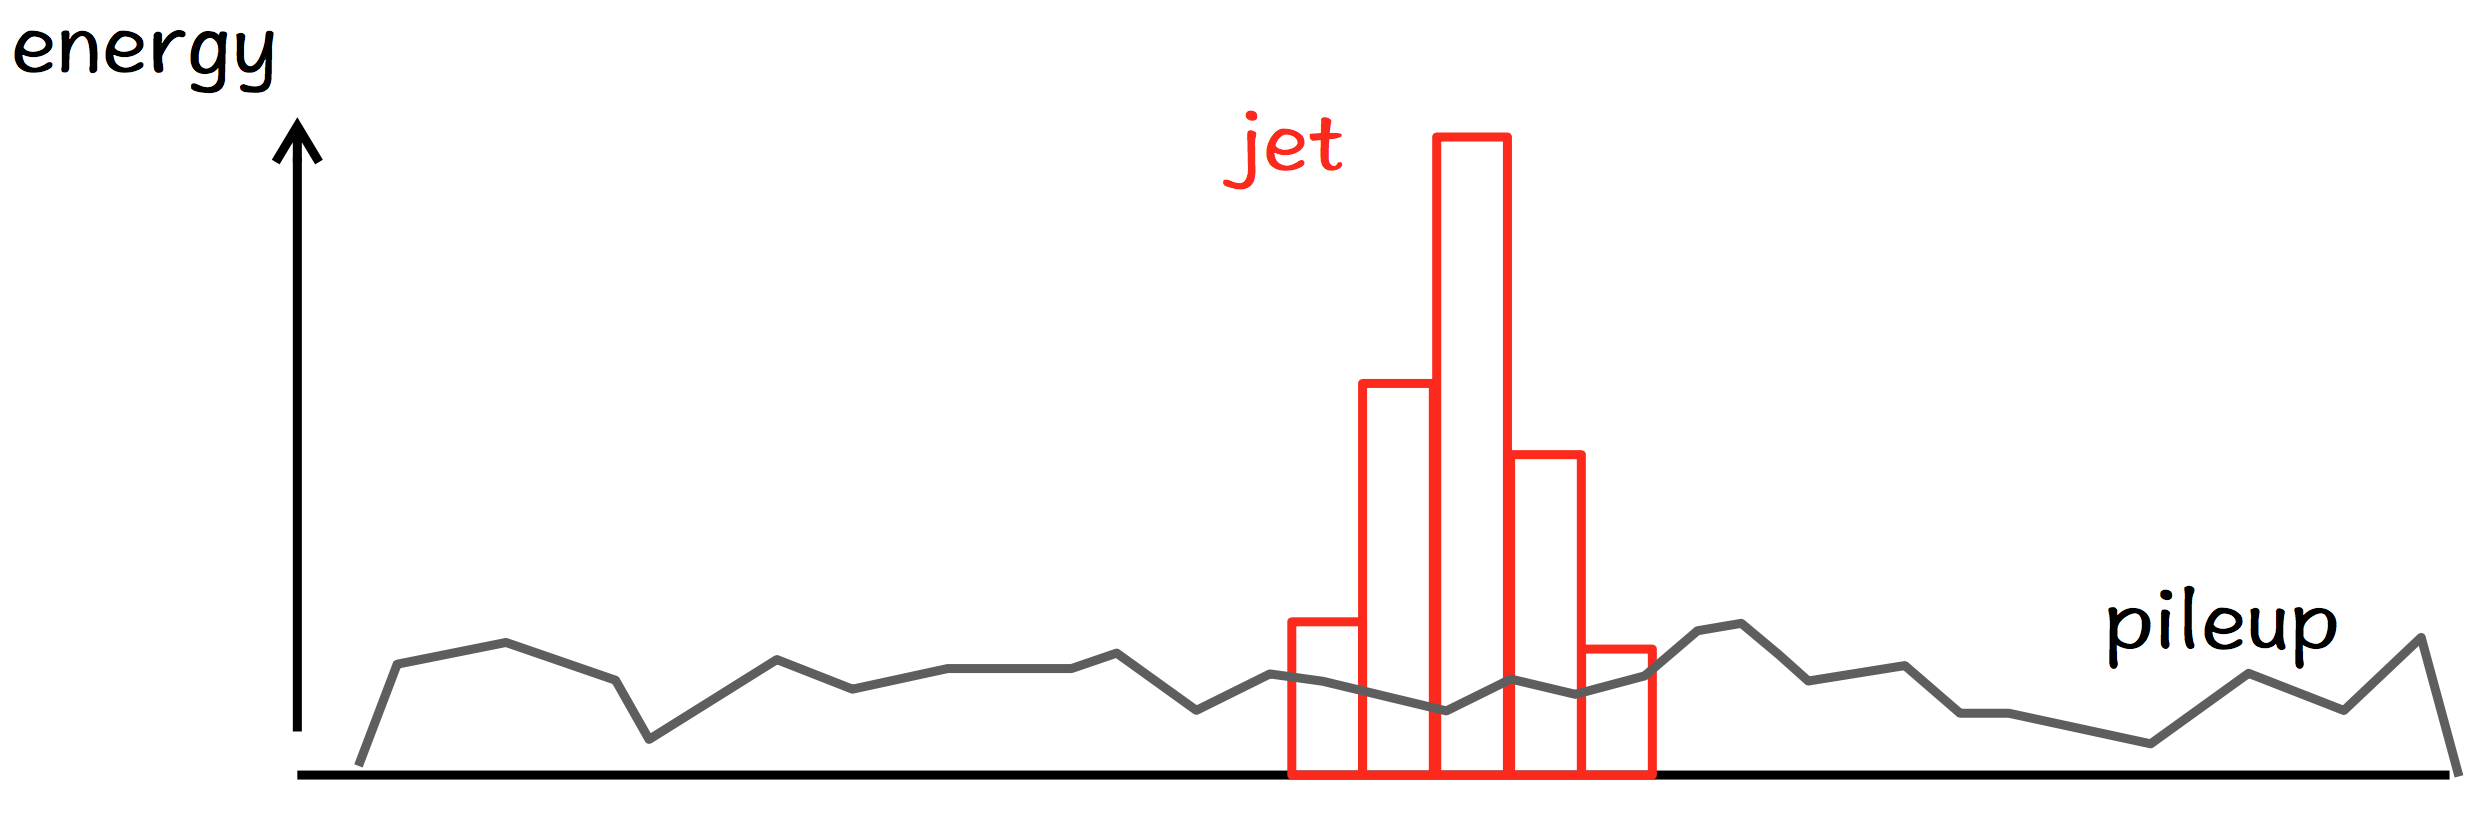
\includegraphics[width=\textwidth]{images/pileup_mitigation/pileup_schematic_2.png}
			}
	\end{textblock}
\end{frame}